\documentclass[10pt]{article}
\usepackage[a4paper,margin=18mm]{geometry}
\usepackage{amsmath,amssymb,booktabs,array,enumitem}
\usepackage[T1]{fontenc}\usepackage{lmodern}
\usepackage{tikz}\usetikzlibrary{shapes.gates.logic.US,positioning,arrows.meta}
\usepackage[hidelinks]{hyperref}
\setlength{\parindent}{0pt}\setlength{\parskip}{4pt}\setlength{\emergencystretch}{2em}
\newcommand{\VDD}{V_{DD}}
\newcommand{\mos}[4]{\begin{scope}[shift={(#1,#2)}]
\draw(0,.23)--(0,-.23);\draw(0,.2)--(.25,.2)--(.25,.5);\draw(0,-.2)--(.25,-.2)--(.25,-.5);
\draw(-.16,.23)--(-.16,-.23);
\ifnum#4=1\draw(-.26,0)circle(.06);\draw(-.7,0)--(-.32,0);\else\draw(-.7,0)--(-.16,0);\fi
\node[anchor=east,font=\scriptsize]at(-.71,0){$#3$};\end{scope}}
\newcommand{\grd}[2]{\draw(#1,#2)--(#1,#2-.12);\draw(#1-.15,#2-.12)--(#1+.15,#2-.12);\draw(#1-.1,#2-.19)--(#1+.1,#2-.19);}
\newcommand{\sourcefigone}{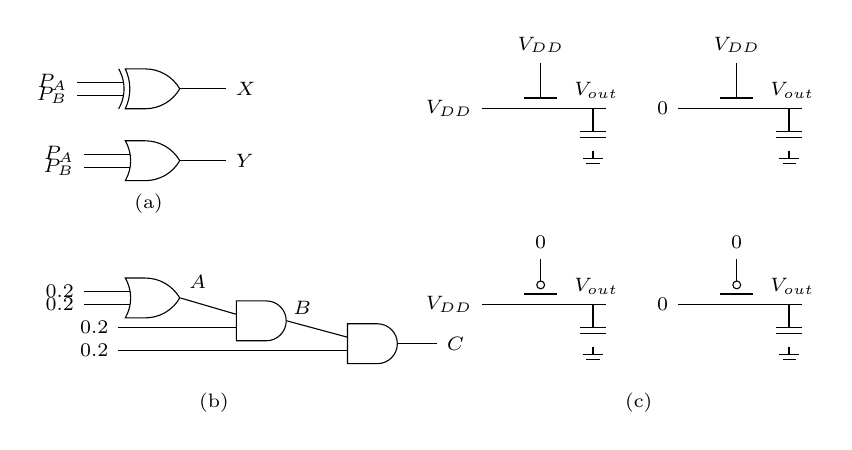
\begin{tikzpicture}[x=.83cm,y=.83cm,font=\scriptsize]
\node[xor gate US,draw,logic gate inputs=nn](x)at(1,4.3){};\node[or gate US,draw,logic gate inputs=nn](y)at(1,3.2){};
\foreach\g in{x,y}{\draw(\g.input 1)--++(-.7,0)node[left]{$P_A$};\draw(\g.input 2)--++(-.7,0)node[left]{$P_B$};}
\draw(x.output)--++(.7,0)node[right]{$X$};\draw(y.output)--++(.7,0)node[right]{$Y$};\node at(1,2.55){(a)};
\node[or gate US,draw,logic gate inputs=nn](a)at(1,1.1){};\node[and gate US,draw,logic gate inputs=nn](b)at(2.7,.75){};\node[and gate US,draw,logic gate inputs=nn](c)at(4.4,.4){};
\draw(a.input 1)--++(-.7,0)node[left]{0.2};\draw(a.input 2)--++(-.7,0)node[left]{0.2};\draw(a.output)--(b.input 1);\draw(b.input 2)--++(-1.8,0)node[left]{0.2};\draw(b.output)--(c.input 1);\draw(c.input 2)--++(-3.5,0)node[left]{0.2};
\node[above]at(1.75,1.1){$A$};\node[above]at(3.35,.7){$B$};\draw(c.output)--++(.6,0)node[right]{$C$};\node at(2,-.5){(b)};
\foreach\x/\yy/\gg/\in/\typ in{7/4/V_{DD}/V_{DD}/0,10/4/V_{DD}/0/0,7/1/0/V_{DD}/1,10/1/0/0/1}{
\draw(\x-.9,\yy)--(\x-.3,\yy) (\x+.3,\yy)--(\x+1,\yy);\draw(\x-.3,\yy)--(\x+.3,\yy);
\draw(\x-.25,\yy+.16)--(\x+.25,\yy+.16);\ifnum\typ=1\draw(\x,\yy+.3)circle(.06);\draw(\x,\yy+.36)--(\x,\yy+.7);\else\draw(\x,\yy+.16)--(\x,\yy+.7);\fi
\node[above]at(\x,\yy+.7){$\gg$};\node[left]at(\x-.9,\yy){$\in$};\node[above]at(\x+.85,\yy){$V_{out}$};\draw(\x+.8,\yy)--(\x+.8,\yy-.35);\draw(\x+.6,\yy-.35)--(\x+1,\yy-.35) (\x+.6,\yy-.45)--(\x+1,\yy-.45);\grd{\x+.8}{\yy-.65}}
\node at(8.5,-.5){(c)};\end{tikzpicture}}
\newcommand{\wirefig}{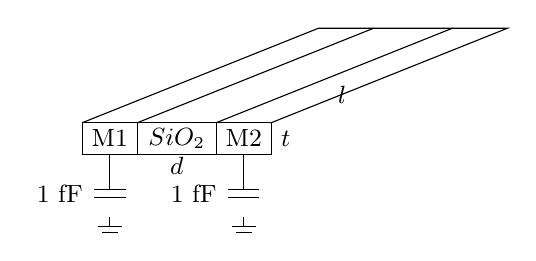
\begin{tikzpicture}[x=1cm,y=1cm,font=\small]
\draw(0,1)rectangle(.7,1.4);\draw(.7,1)rectangle(1.7,1.4);\draw(1.7,1)rectangle(2.4,1.4);
\draw(0,1.4)--(3,2.6)--(5.4,2.6)--(2.4,1.4);\draw(.7,1.4)--(3.7,2.6) (1.7,1.4)--(4.7,2.6);
\node at(.35,1.2){M1};\node at(1.2,1.2){$SiO_2$};\node at(2.05,1.2){M2};\node at(3.3,1.75){$l$};\node[right]at(2.4,1.2){$t$};\node at(1.2,.85){$d$};
\foreach\x in{.35,2.05}{\draw(\x,1)--(\x,.55);\draw(\x-.2,.55)--(\x+.2,.55) (\x-.2,.45)--(\x+.2,.45);\grd{\x}{.2}\node[left]at(\x-.22,.5){1 fF};}\end{tikzpicture}}
\newcommand{\chainsfig}{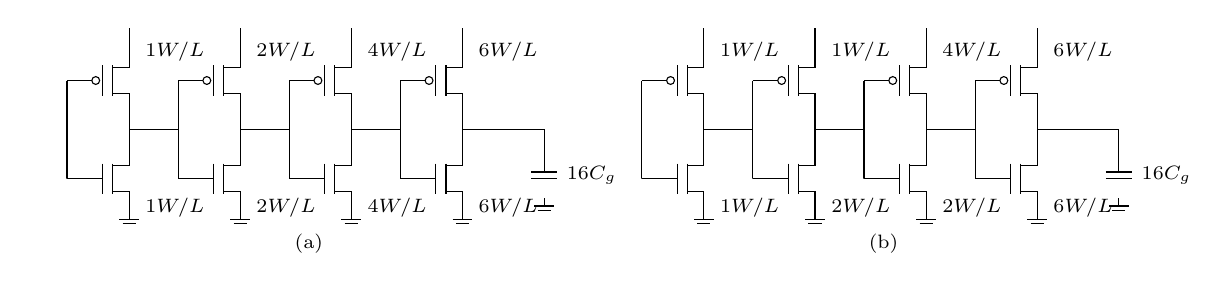
\begin{tikzpicture}[x=.83cm,y=.83cm,font=\scriptsize]
\begin{scope}[xshift=0cm]
\mos{0.0}{2.5}{\phantom{X}}{1}\mos{0.0}{1}{\phantom{X}}{0}
\draw(0.25,3)--(0.25,3.3);\draw(0.25,2)--(0.25,1.5);\grd{0.25}{.5}
\draw(-0.7,2.5)--(-0.7,1)--(-0.7,1.75);
\node[above right]at(0.35,2.65){$1W/L$};\node[below right]at(0.35,.85){$1W/L$};
\draw(0.25,1.75)--(1.0,1.75);
\mos{1.7}{2.5}{\phantom{X}}{1}\mos{1.7}{1}{\phantom{X}}{0}
\draw(1.95,3)--(1.95,3.3);\draw(1.95,2)--(1.95,1.5);\grd{1.95}{.5}
\draw(1.0,2.5)--(1.0,1)--(1.0,1.75);
\node[above right]at(2.05,2.65){$2W/L$};\node[below right]at(2.05,.85){$2W/L$};
\draw(1.95,1.75)--(2.7,1.75);
\mos{3.4}{2.5}{\phantom{X}}{1}\mos{3.4}{1}{\phantom{X}}{0}
\draw(3.65,3)--(3.65,3.3);\draw(3.65,2)--(3.65,1.5);\grd{3.65}{.5}
\draw(2.7,2.5)--(2.7,1)--(2.7,1.75);
\node[above right]at(3.75,2.65){$4W/L$};\node[below right]at(3.75,.85){$4W/L$};
\draw(3.65,1.75)--(4.4,1.75);
\mos{5.1}{2.5}{\phantom{X}}{1}\mos{5.1}{1}{\phantom{X}}{0}
\draw(5.35,3)--(5.35,3.3);\draw(5.35,2)--(5.35,1.5);\grd{5.35}{.5}
\draw(4.3999999999999995,2.5)--(4.3999999999999995,1)--(4.3999999999999995,1.75);
\node[above right]at(5.449999999999999,2.65){$6W/L$};\node[below right]at(5.449999999999999,.85){$6W/L$};
\draw(5.35,1.75)--(6.6,1.75)--(6.6,1.1);\draw(6.4,1.1)--(6.8,1.1) (6.4,1)--(6.8,1);\grd{6.6}{.7}\node[right]at(6.8,1.05){$16C_g$};
\node at(3,0){(a)};
\end{scope}
\begin{scope}[xshift=7.3cm]
\mos{0.0}{2.5}{\phantom{X}}{1}\mos{0.0}{1}{\phantom{X}}{0}
\draw(0.25,3)--(0.25,3.3);\draw(0.25,2)--(0.25,1.5);\grd{0.25}{.5}
\draw(-0.7,2.5)--(-0.7,1)--(-0.7,1.75);
\node[above right]at(0.35,2.65){$1W/L$};\node[below right]at(0.35,.85){$1W/L$};
\draw(0.25,1.75)--(1.0,1.75);
\mos{1.7}{2.5}{\phantom{X}}{1}\mos{1.7}{1}{\phantom{X}}{0}
\draw(1.95,3)--(1.95,3.3);\draw(1.95,2)--(1.95,1.5);\grd{1.95}{.5}
\draw(1.0,2.5)--(1.0,1)--(1.0,1.75);
\node[above right]at(2.05,2.65){$1W/L$};\node[below right]at(2.05,.85){$2W/L$};
\draw(1.95,1.75)--(2.7,1.75);
\mos{3.4}{2.5}{\phantom{X}}{1}\mos{3.4}{1}{\phantom{X}}{0}
\draw(3.65,3)--(3.65,3.3);\draw(3.65,2)--(3.65,1.5);\grd{3.65}{.5}
\draw(2.7,2.5)--(2.7,1)--(2.7,1.75);
\node[above right]at(3.75,2.65){$4W/L$};\node[below right]at(3.75,.85){$2W/L$};
\draw(3.65,1.75)--(4.4,1.75);
\mos{5.1}{2.5}{\phantom{X}}{1}\mos{5.1}{1}{\phantom{X}}{0}
\draw(5.35,3)--(5.35,3.3);\draw(5.35,2)--(5.35,1.5);\grd{5.35}{.5}
\draw(4.3999999999999995,2.5)--(4.3999999999999995,1)--(4.3999999999999995,1.75);
\node[above right]at(5.449999999999999,2.65){$6W/L$};\node[below right]at(5.449999999999999,.85){$6W/L$};
\draw(5.35,1.75)--(6.6,1.75)--(6.6,1.1);\draw(6.4,1.1)--(6.8,1.1) (6.4,1)--(6.8,1);\grd{6.6}{.7}\node[right]at(6.8,1.05){$16C_g$};
\node at(3,0){(b)};
\end{scope}
\end{tikzpicture}}
\newcommand{\qsevenfig}{\begin{tikzpicture}[x=1cm,y=.85cm,font=\small]
\mos{2}{6}{A}{1}\draw(2.25,6.5)--(2.25,6.9)node[above]{$V_{DD}$};
\draw(2.25,5.5)--(.75,5.5)--(.75,4.5) (2.25,5.5)--(3.75,5.5)--(3.75,5);
\mos{.5}{4}{B}{1}\mos{3.5}{4.5}{C}{1}\mos{3.5}{3}{D}{1}\draw(3.75,4)--(3.75,3.5);
\draw(.75,3.5)--(.75,2.3)--(3.75,2.3)--(3.75,2.5);\draw(2.25,2.3)--(5.2,2.3)node[right]{$F$};
\draw(2.25,2.3)--(.25,2.3)--(.25,1.4);\mos{0}{.9}{A}{0}\draw(.25,.4)--(.25,-1.1);
\draw(2.25,2.3)--(2.25,2);\mos{2}{1.5}{B}{0}\draw(2.25,1)--(2.25,.7)--(1.5,.7)--(1.5,.4) (2.25,.7)--(3.25,.7)--(3.25,.4);
\mos{1.25}{-.1}{C}{0}\mos{3}{-.1}{D}{0}\draw(1.5,-.6)--(1.5,-1.1)--(.25,-1.1) (3.25,-.6)--(3.25,-1.1)--(1.5,-1.1);\grd{1.5}{-1.1}
\end{tikzpicture}}
\newcommand{\aoifig}{\begin{tikzpicture}[x=1cm,y=.8cm,font=\small]
\mos{0}{4}{a}{1}\mos{2}{4.7}{b}{1}\mos{2}{3.3}{c}{1}\draw(.25,4.5)--(.25,5.4)--(2.25,5.4)--(2.25,5.2);\node[above]at(1.25,5.4){$V_{DD}$};\draw(2.25,4.2)--(2.25,3.8);
\draw(.25,3.5)--(.25,2.6)--(2.25,2.6)--(2.25,2.8);\draw(1.25,2.6)--(3.5,2.6)node[right]{$f$};
\mos{1}{2}{a}{0}\draw(1.25,2.6)--(1.25,2.5);\draw(1.25,1.5)--(.25,1.5)--(.25,1.2) (1.25,1.5)--(2.25,1.5)--(2.25,1.2);
\mos{0}{.7}{b}{0}\mos{2}{.7}{c}{0}\draw(.25,.2)--(.25,-.2)--(2.25,-.2)--(2.25,.2);\grd{1.25}{-.2}\end{tikzpicture}}
\begin{document}
\begin{center}{\large\bfseries EE3032 Introduction to VLSI Design -- Midterm}\end{center}
\textbf{Fall 2007.} Printed percentages sum to 110\%, not 100\%; all allocations are preserved.
\textbf{1. (40\%)} Answer the following problems.
\begin{enumerate}[label=(\alph*),leftmargin=7mm,itemsep=1pt]
\item Draw a CMOS transistor-level schematic realizing the Boolean function $f=\overline{a(b+c)}$. (4\%)
\item List the process for transferring the mask pattern to the surface of a silicon region. (4\%)
\item List three approaches for increasing the performance of a CMOS circuit. (6\%)
\item List two latchup prevention approaches. (4\%)
\item List three principles for reducing the switching power of a CMOS circuit. (6\%)
\item Explain the purpose of design rules in VLSI design. (4\%)
\item Explain what the body effect is. (4\%)
\item Explain why adding a guard ring can reduce the latchup effect. (4\%)
\item Explain the energy consumption of an inverter when the inverter performs a switching. (4\%)
\end{enumerate}

\textbf{2. (10\%)} (a) Design an 8-to-1 multiplexer using pass transistor logic. (5\%) (b) Design a two-input exclusive-or (XOR) gate using CMOS transmission gates. (5\%)

\textbf{3. (20\%)} Complete the following problems.
\begin{enumerate}[label=(\alph*),leftmargin=7mm]
\item Figure 1(a) shows the XOR and OR gate. Assume that $P_A$ and $P_B$ are the mutually independent signal probabilities of inputs $A$ and $B$ to be at ``1''. Express the $P_{0\to1}$ of $X$ and $Y$. (5\%)
\item Figure 1(b) shows a circuit with one OR and two AND gates. Assume the 1's probabilities of inputs all are 0.2. Calculate the $P_{0\to1}$ of $A$, $B$, and $C$. (10\%)
\item Figure 1(c) shows the pass transistor logics with NMOS and PMOS. Level the source and drain of the circuits, and calculate $V_{out}$ of the circuits. (5\%)
\end{enumerate}
\begin{center}\sourcefigone\\Figure 1: (a) primitive gates (b) cascade design (c) pass transistors.\end{center}
\newpage
\begin{center}\wirefig\\Figure 2: Two parallel wires.\end{center}
\textbf{4. (10\%)} There are two parallel wires, M1 and M2, as shown in Figure 2. Assume that $\epsilon_{SiO_2}=5\times10^{-14}\,\mathrm{F/cm}$, $d=1\,\mu\mathrm m$, $t=1\,\mu\mathrm m$, and $l=100\,\mu\mathrm m$. If M2 is floating and M1 has a 0 V to 1.8 V transition, how much crosstalk noise will be coupled on M2?

\textbf{5. (10\%)} Figure 3 depicts two designs of inverter chains. Assume that the equivalent resistance of a minimum size $W/L$ NMOS is $R$ and $\mu_n=2\mu_p$. The gate capacitance of a $W/L$ transistor is $C_g$. Also, the parasitic capacitances of drain/source and wires are neglected. Which inverter chain consumes lower short-circuit power? Explain your answer.
\begin{center}\chainsfig\\Figure 3: Inverter chains.\end{center}
\textbf{6. (10\%)} Suppose that the signal delay on an interconnect of length $50\,\mu\mathrm m$ is known to be $0.13\,\mathrm{ps}$. If the line is increased to $100\,\mu\mathrm m$, then what is the delay of the line? (4\%) If you can insert an inverter in the $100\,\mu\mathrm m$ interconnect and the inverter delay is $0.2\,\mathrm{ps}$, where should the inverter be inserted such that the wire delay is minimized, and how much is the delay of the interconnect with buffer insertion? (6\%)

\textbf{7. (10\%)} Size the transistors in the circuit shown below that implements a function $F=\overline{A+B(C+D)}$ so that its worst case current driving capability is equivalent to that of an inverter with $W_p/L_p=10\lambda/2\lambda=5$ and $W_n/L_n=4\lambda/2\lambda=2$. Assume that the channel length of all transistors is fixed at $2\lambda$.
\newpage\begin{center}\qsevenfig\end{center}
\vfill\small Editable reconstruction of all three source pages. Printed questions, values, connections and percentage labels are retained. The very small ps delays are reproduced as printed; no unit correction is assumed.
\end{document}
